%!TEX root = ../thesis.tex
%*******************************************************************************
%**************************** Introductory Chapter *****************************
%*******************************************************************************

\chapter{Introduction} %Title of first chapter

\ifpdf
    \graphicspath{{Chapter0/Figs/Raster/}{Chapter0/Figs/PDF/}{Chapter0/Figs/}}
\else
    \graphicspath{{Chapter0/Figs/Vector/}{Chapter0/Figs/}}
\fi

%********************************** %First Section  **************************************
\section{Motivation}
Hominids have always manipulated and altered their environment. Ancient people replanted wild flora and helped drive various megafauna such as woolly mammoth and steppe bison to extinction \cite{Mann2015} \cite{Pushkina2008}. Today, we are still changing our surroundings, but at a historically unprecedented rate. Paul Crutzen popularised the term anthropocene in the early 2000s, defining it as the current geological period of Earth's existence, one where humanity has a significant on the planet's various systems, in many ways outcompeting natural processes \cite{Crutzen2006}. Our rapacious desire for resources has felled forests, excavated vast holes in the Earth, driven countless species extinct and burnt fossil fuels at tremendous scale, releasing greenhouse gases (GHG) including carbon dioxide into the atmosphere. This last process has driven atmospheric CO$_{2}$ concentrations from 280ppm to 410ppm in two centuries \cite{}. The rate of accumulation is currently 2ppm and accelerating \cite{}. This accumulation of GHGs is driving climate change, leading to an atmospheric temperature increase of X since Y \cite{}. The consequences of the increased energy retained in the Earth system are many and varied. Sea levels have risen by X in Y years \cite{}. Arctic sea ice coverage has receeded by X since Y \cite{}. Oceans have warmed and acidified, resulting in coral loss of X \cite{}. The condition of the planet will undoubtedly continue to deteriorate in the coming decades. It is highly likely that increasingly frequent droughts will engender conflict \cite{}. Tropical diseases will spread from equatorial regions to the warming temperate zones \cite{}. Extreme weather events will probably become more frequent \cite{}. These conditions are now `baked-in' and will happen regardless of humanities efforts to avert them. This is because there is a long lag between addition of GHG to the atmosphere and a new temperature equilibrium being reached \cite{}. Two degrees of atmospheric warming over pre-industrial temperature is now extremely likely \cite{}. We must now mitigate the risks posed by our changed and changing planet and act to prevent warming worse than two degrees, for the consequences of further increases are dire \cite{}.

% Reference David McKay? Check his figures for consumption and correct if necessary
The main sources of GHG emission that humans are responsible for are combustion of fossil fuels for heat (industrial and domestic heating and cement production), transport (internal combustion engines and jet engines) and electricity production (typically with a boiler and steam turbine) and agriculture (deforestation and animals' methane production) \cite{}. We must rapidly reduce our GHG emission from current levels to near-zero or even negative rates \cite{}. In order to achieve this, heating, transport and electricity production must be decarbonised. Unfortunately, removing fossil fuels from heating and transport is most likely to be achieved with their electrification. This, coupled with a growing population and desire for increasing material living standards, means low-carbon electricity demand is going to dramatically increase in the near future \cite{}. 

%\cite{Zalasiewicz2017}

Low-carbon electricity production is currently produced from nuclear fission and renewables such as solar photovoltaic, solar thermal, wind, hydro, tidal, geothermal and biofuels. The acronym WWS (Wind, Water and Solar) summarises the renewable methods with greatest potential for widespread adoption. 

While nuclear fission is very safe by the metric of energy produced per death caused \cite{} it has spawned several major accidents, suffers from issues of public acceptability, radioactive waste storage and, more recently, construction cost. Additionally, the current trend for an open fuel cycle where nuclear fuel is not reprocessed and then reused is wasteful and drastically limits the potential of nuclear fission at scale \cite{}. WWS have tremendous potential and are currently gaining market share, with costs falling rapidly. For instance, some utilities are now bidding to supply electricity for as little as 1.2p per $kW \cdot h$ \cite{}. For comparison, the Hinkley Point C nuclear fission plant will have a minimum supply price of 9.25p per $kW \cdot h$ \cite{}. Unfortunately, intermittancy is a significant problem for WWS, specifically wind and solar. Much work is required to fully exploit its potential: drastic improvements in energy storage methods, a commensurate deployment of such technology, intelligent demand optimisation and improved distribution networks. Even then, it is unclear if WWS and/or nuclear fission could provide enough electricity for our future society \cite{}. A potential future alternative to both WWS and nuclear fission is nuclear fusion, the process of combining nuclei by which stars shine.

% Rebuttal to those Californian 100% WWS papers? 

\section{Nuclear fusion}
...

\subsection{Discovery}
Einstein's energy-mass equivalence, $E=mc^{2}$ led Arthur Eddington to hypothesise that the energy released by the sun was through the fusion of hydrogen nuclei into helium nuclei. Classical predictions of the temperature required for the sun's power output did not match observations. Indeed, the temperatures observed seemed too low for nuclei to overcome the Coulomb energy barrier - the repulsive force experienced by two nuclei. The development of a theory of quantum tunnelling in the late 1920s by Gamow and others, predicted thermonuclear temperatures in accordance with observations of the sun. 

In the 1930s Mark Oliphant, Paul Harteck and Ernest Rutherford conducted particle beam experiments, bombarding various targets with deuterons. After several less interesting combinations, they observed ``on bombarding heavy hydrogen with diplons\footnote{Diplon was a contemporary name for what we now call deuterium} an enormous effect was produced`` \cite{}. This included the emission of high energy neutrons. %https://www.chemteam.info/Chem-History/Rutherford-1934b/Rutherford-1934b.html

\subsection{Possible reactions to harness}
Trying to fuse nuclei is difficult, as scattering via the Coulomb force is far more likely than fusion for all potential reactants. This Coulomb barrier is proportional to the product of the charges of the reactants as shown in equation \ref{eq:coulomb}, where $k_{e}$ is the Coulomb constant, $Z_{i}$ the respective atomic numbers, $e$ the charge on the electron and $r$, the interaction radius.

\begin{equation}
  \label{eq:coulomb}
  U_{coul} = k_{e}\frac{Z_{1}Z_{2}e^{2}}{r}
\end{equation}

Given this, it is only plausible to employ light nuclei for energy production. Of the light nuclei, certain reactions are more likely than others, with a greater cross-section for a given collision energy. They are shown in table \ref{tab:fuels} below.

\begin{table}[h]
\centering
\caption{Comparison of potential fusion fuels. The Q-value is the combined kinetic energy of the reaction products. {\sigma} is the cross-section of the reaction at a given energy, with centre-of-mass energies.}
\label{tab:fuels}
\begin{tabular}{@{}lllll@{}}
\toprule
Fuel          & Products          & Q-value (MeV) & \sigma (10 keV) \mathrm{(barn)} & \sigma (100 keV) \mathrm{(barn)} \\ \midrule
D + T         & \alpha + n        & 17.6          & $2.72\times10^{-2}$    & 3.43                    \\
D + D         & T + p             & 4.04          & $2.81\times10^{-4}$    & $3.3\times10^{-2}$      \\
D + D         & $^{3}$He + n      & 3.27          & $2.78\times10^{-4}$    & $3.7\times10^{-2}$      \\
D + $^{3}$He  & \alpha + p        & 18.3          & $2.2\times10^{-7}$     & 0.1                     \\
p + $^{11}$B  & 3\alpha           & 8.68          & $4.6\times10^{-17}$    & $3\times10^{-4}$        \\ \bottomrule
\end{tabular}
\end{table}

At an energy of 10 keV the D-T fusion reaction has a likelihood 100-fold of the next easiest reactions. It also has a large Q-value, with 17.6 MeV of binding energy released by the reconfiguration of the fuel nucleons. D-$^{3}$He and p-$^{11}$B fuels are aneutronic, with only charged products. These fuels would obviate several difficult problems associated with D-T fusion, arising from the energetic emitted neutrons. Unfortunately these aneutronic fuels require extraordinary temperatures to fuse. D-T fuel is currently envisioned for the majority of fusion concepts.

\subsection{Development}
The subsequent decade saw the invention and development of so-called `pinch` fusion concepts. As a current flows through a tube of conducting medium (such as a plasma) the magnetic field generated acts in tandem with the current to crush the material to a filament by a Lorentz, or $\mathbf{j \times B}$ force. This is a kind of confinement, momentarily holding plasma ions in an increased density state. By bending a tube into a toroidal shape, matter might be circulated about a device, permanently confined. In reality, the gradient of the electric field across the torus acts to break confinement and lose material. 

In the 1950s, the pinch concept was developed by Soviet scientists Sakharov and Tamm, into the tokamak. This was similar to previous designs of toroidal pinch machines, such as the British ZETA, but the relative strength of fields was different. Rather than having the dominant field be produced by the plasma current, in a tokamak the dominant field is generated by the toroidal field coils which wrap around the toroidal plasma chamber. Over the coming decades this would prove to be a more stable confinement system than other approaches. 

Throughout the rest of the 20th century, the tokamak concept came to dominate magnetic confinement fusion research. Plasma physicists around the world continued to design devices and plasma scenarios which attempt to avoid plasma instabilities and maximise the plasma triple product, developed from Lawson's criterion \cite{lawson1955}. The triple product, $nT\tau_{E}$, is the product of the plasma density, temperature and energy confinement time, respectively. Figure \ref{fig:triple_product} shows a plot of this performance metric against time. One can see the progress in relation to the well known Moore's Law in computing performance per unit cost and the beam energy of various particle colliders. Viewed in this way, fusion power has achieved remarkable progress across the decades (logarithmic and temporal).

\begin{figure}
%  \figuretitle{}
  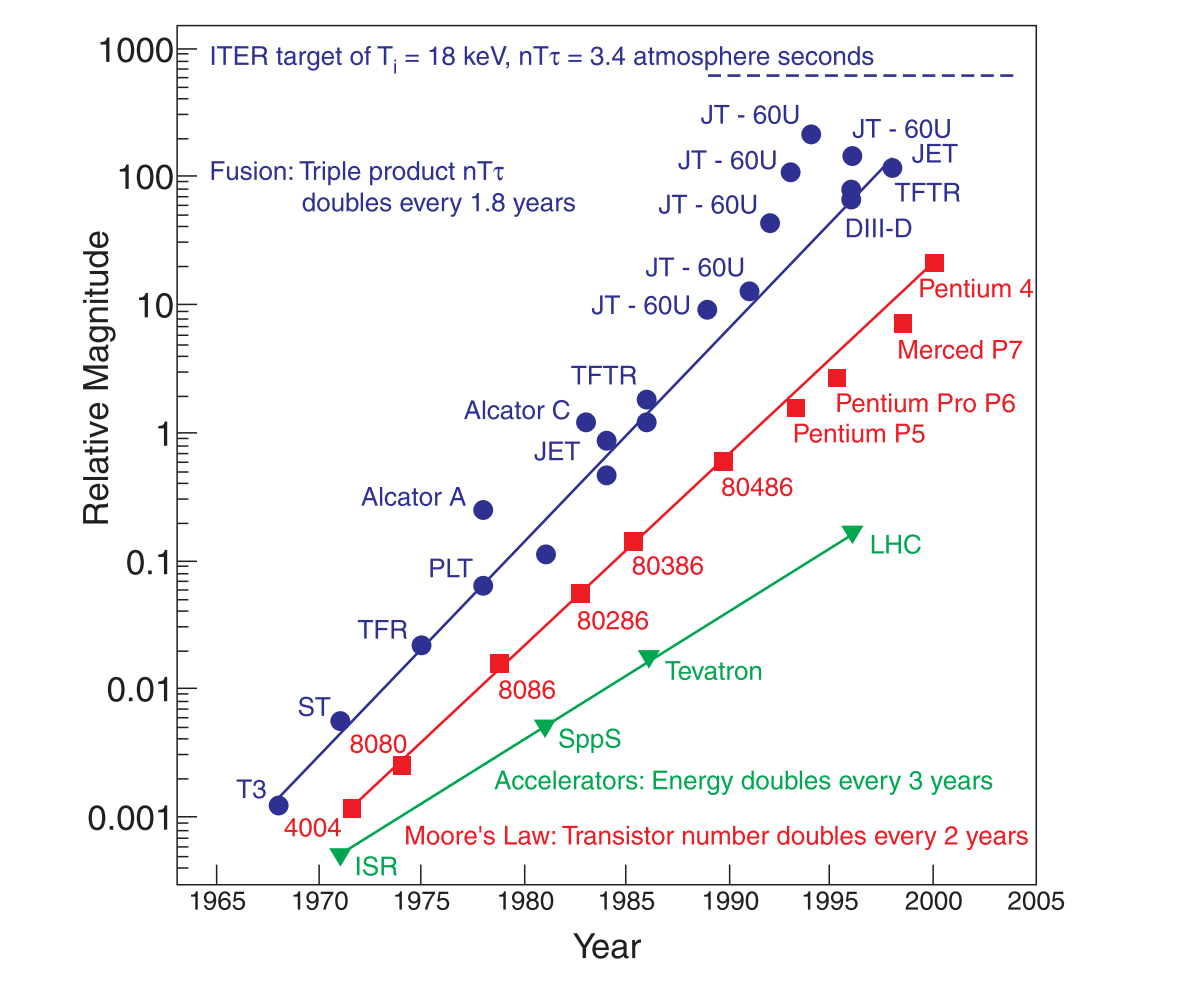
\includegraphics[width=0.47\textwidth]{triple_product.png}
  \caption{Fusion triple product achieved plotted against time. Similar progress measures for computing and particle physics are also shown. }
  \label{fig:triple_product}
\end{figure}

\subsection{Future plans}

\section{Radiation-matter interactions}
Nuclear fusion gives rise to various energetic particles. The reaction most likely to result in the first fusion reactors is D + T \rightarrow $^{4}$He + n + 17.6 MeV. The neutrons are emitted with $\frac{4}{5}$ of the total energy liberated, to give 14.1 MeV of kinetic energy. 

Photons are constantly generated in a tokamak plasma. Low energy photons are of characteristic energy are created through the excitation and de-excitation of atomic electrons, while Bremsstrahlung radiation arised from the acceleration of charged particles.

This mixed radiation field is then further complicated by numerous interaction process, as neutrons and photons from the plasma interact with the device. What follows is a short primer on the possible interaction processes.

\subsection{Neutron}
The neutron is a sub-atomic particle of mass $1.674927471(21)\times10^{-27}$kg \cite{}, composed of three quarks. It can exist as part of a nucleus or unbound, where it has a mean lifetime of $881.5(15)$s \cite{}. While it is itself uncharged it can produce ionising radiation through interactions with other matter. These reactions are via the strong, weak, graviational and electromagnetic\footnote{While the neutron has zero electric charge, it does have a magnetic moment, and is therefore acted upon by electromagnetic fields.} forces. 

When neutrons undergo collisions, the ensuing process is strongly dependent on the combined energy of the reactants. Energies can theoretically range from ... to ... . Shown below is a diagram of the relevant processes across the energy domain.

... fig ...

\subsubsection{Diffraction}

\subsubsection{Elastic scattering}

\subsubsection{Nuclear reactions}

\paragraph{Inelastic scattering}

\paragraph{Fission}

\paragraph{Radiative capture}

\paragraph{Multiplication}

\paragraph{Other reactions}

\subsection{Gamma}
The gamma ray, or photon, is a 

\subsubsection{Photoelectric}

\subsubsection{Compton scattering}

\subsubsection{Pair production}

\section{Sources of uncertainty in fusion neutronics}
The sources of uncertainty in fusion neutronics are many and varied. Currently envisioned fusion reactors such as ITER rank as some of the most complex machines ever. Their multitude of components, diversity of materials and range of scales make simulating their operation challenging. While the devices themselves are large and difficult to model, introducing uncertainties into calculations, other kinds of uncertainty are inherent in the practice of neutronics more generally. Knowledge of nuclear physics, colloquially referred to as `nuclear data' (ND) is incomplete and uncertain for a variety of reasons. These include:  

\section{Implications of current uncertainties}

\section{Thesis outline}
